\documentclass{llncs}
\usepackage{graphicx}
\usepackage{booktabs}
\usepackage{amsmath}
\usepackage{hyperref}

\setlength{\textfloatsep}{6pt plus 1pt minus 2pt}
\setlength{\intextsep}{4pt plus 1pt minus 2pt}
\setlength{\abovecaptionskip}{3pt}
\setlength{\belowcaptionskip}{1pt}
\renewcommand{\arraystretch}{0.9}

\begin{document}

\title{Repurposing Beyond the Nearest Analog: Debiasing Drug-Indication Models Against Chemical-Similarity Shortcuts}

\author{Rishik Kondadadi\inst{1} \and John Ortega\inst{2}}
\institute{University of Minnesota \and Northeastern University}

\maketitle

\begin{abstract}
A zero-training nearest-neighbor chemical-similarity search already predicts a drug's indication well when that drug has a close analog among known treatments. Across nine therapeutic classes in our data it averages 0.866 AUROC with no training at all. Its accuracy collapses, however, on drugs with no close known analog: down to 0.21--0.46 AUROC on four of the nine classes. That is exactly where a repurposing model needs to work. We adapt DebiasedDTA, a guide/predictor reweighting scheme built for drug-target binding-affinity prediction, to drug-indication prediction. Our three-view model combines chemical structure, L1000 expression, and a text encoding of each drug's target function, targeting signal this similarity shortcut cannot explain.

On epilepsy, the class that motivated this study, debiasing gives a +0.116 cold-bucket AUROC benefit over an otherwise identical undebiased model, under the ChEMBL label this benchmark is built on. Two independent checks corroborate it. A biological-interpretation check on a field never seen in training, the Repurposing Hub's mechanism-of-action label, agrees from an independent angle: the debiased model's top cold-bucket candidates are enriched 23-fold for plausible antiseizure mechanisms, a further lift over the already-large undebiased enrichment. A quintile-based robustness check reproduces a comparable delta on a different split, ruling out the tertile cutoff as an artifact. Two further checks narrow the claim. An external repoDB comparison is underpowered, only 5 compounds overlap, and does not reproduce the delta. A better-powered check, extending the pool to 56 epilepsy positives, shows the benefit holds for candidates with a complete three-view profile and collapses on new candidates lacking an expression profile. We report the epilepsy delta as real on the pool it was built for, not yet shown to extend beyond it.

Beyond epilepsy, the picture is honestly mixed, not a uniform win. Debiasing gives a small benefit on one further class and a modest cost on two more. The remaining five classes show no usable signal either way, because their cold buckets simply contain too few positives per fold to support any claim. We report this cross-class picture directly rather than smoothing it into one pooled number.

Two further findings support the paper's broader case for evaluation care in this setting, though neither is the paper's main result. Adapting two debiasing methods from the literature, DRDM and TAPB, to this task shows our model still holds the best point estimate. But the comparison also surfaces that one of them looks strong mainly because of joint multi-indication training, not its own correction, a transferable pitfall for anyone benchmarking an adapted debiasing baseline. Separately, a leakage audit justifies why literature about the drug itself cannot be used as a feature: PubMed abstracts predict a drug's eventual indication at 0.96 AUROC even before approval, almost entirely through mentions of other same-class drugs.
\end{abstract}

\section{Introduction}
Drug repurposing models are usually scored on how well they rank known treatments above everything else. A large part of that score is explained by chemistry alone. In our data, a nearest-neighbor search over ECFP4 fingerprints already averages 0.866 AUROC across nine therapeutic classes (epilepsy, depression, antipsychotics, antibacterials, antidiabetics, antineoplastics, lipid-lowering drugs, NSAIDs, and antihypertensives), with no training at all: it simply scores each candidate by its maximum Tanimoto similarity to a known positive. This is not a trivial baseline to beat, because much of it is not wrong. Drugs really do cluster by mechanism, and a new analog of a known treatment really is a reasonable candidate. The question this paper asks is what happens on the drugs that do not have a close known analog. Those are the ones a repurposing model is actually for.

On that subset the picture changes sharply. We stratify each class's test compounds by similarity to the training positives and look at the bottom tertile. There, the nearest-neighbor search's AUROC falls to 0.21 on NSAIDs, 0.43 on epilepsy, 0.44 on antibacterials, and 0.46 on antineoplastics, each close to or below chance. A model that only reproduces this shortcut fails exactly where repurposing matters most. We ask whether a model can be trained specifically against this known bias, using a guide/predictor reweighting scheme from DebiasedDTA~\cite{ozcelik2023debiaseddta}. DebiasedDTA was originally built to debias binding-affinity prediction against chemical similarity; we retarget it here at a different bias, chemical analog similarity to known indications rather than structure-activity relationships, and a different task, indication classification rather than affinity regression. We also add two further signal sources beyond chemistry: L1000 gene-expression profiles, and a text view encoding what each drug's known target does, from UniProt function descriptions via a biomedical language model. That text view connects drugs through target function even when no training example saw that exact target with a positive label.

Section~\ref{sec:experiments} shows this fix working on epilepsy, the class that motivated the study, and corroborated two independent ways: a mechanism-of-action enrichment check and a quintile-split robustness check. The other eight classes show a more mixed picture, which we report directly rather than smoothing into one pooled number. Two further results support the paper's broader argument for evaluation care without being its main result: an adapted-baseline comparison that surfaces a reproducibility pitfall in one competing method, and a leakage audit explaining a feature we deliberately excluded.

A model that uses text about the drug itself, rather than about its target, would appear to solve this problem trivially. That appearance is incorrect. PubMed abstracts mentioning a drug predict its eventual indication at 0.96 AUROC even when restricted to literature published before that drug's own approval date. Masking the obvious disease-defining terms barely changes this: the remaining signal is mentions of other, already-approved drugs in the same class. We exclude this feature deliberately and report the audit that justifies doing so.

\section{Related Work}

\paragraph{Debiasing drug-target and drug-repurposing models.}
DebiasedDTA~\cite{ozcelik2023debiaseddta} introduced a two-stage guide/predictor framework for drug-target affinity prediction. A low-capacity guide is cross-validated to produce per-sample importance coefficients, and the predictor trains with sample weights interpolating from uniform toward those. It was evaluated only on binding-affinity regression; its own discussion flags extension to other tasks as open. A companion release, pydebiaseddta~\cite{barsbey2023pydebiaseddta}, made the framework reusable with arbitrary guide/predictor pairs. TAPB~\cite{tapb2025} debiases drug-target interaction prediction against protein-target popularity via an interventional correction built on a SMILES-BERT encoder and frozen ESM-2 target embeddings, with no analogue here. The closest repositioning work is DRDM~\cite{meng2025drdm}, which reweights drug-disease graph edges during GNN training against node-degree bias, on benchmarks far denser than ours. Neither transfers as-is. Section~\ref{sec:baselines} therefore implements and tests each mechanism adapted to our data, rather than only noting the mismatch. We know of no prior work using a chemical-similarity nearest-neighbor guide for indication prediction.

\paragraph{Chemical similarity as an evaluation confound.}
Train-test compound similarity inflates apparent molecular-prediction performance. Scaffold splits still leave substantial similarity~\cite{scaffoldsplits2024}, and similarity-aware evaluation shows standard splits dominate reported performance~\cite{similarityaware2025}. Guney~\cite{guney2017reproducible} made this argument for drug repurposing specifically, showing many reported successes reduce to near-duplicate recovery. A companion study from this group~\cite{kondadadi2026ichiaudit} audits this confound on the same library but proposes no model; this paper targets a training-time correction instead. The activity-cliff literature~\cite{vantilborg2022activitycliffs} shows similarity can also actively mislead, not just fail to inform.
\paragraph{Gene-expression and protein-function-text views.}
LINCS L1000~\cite{subramanian2017l1000} gene-expression signatures are widely used for repurposing, including models predicting L1000-style profiles for unmeasured compounds~\cite{pham2021deepce}. TxGNN~\cite{huang2024txgnn} is a prominent recent repurposing baseline, but its zero-shot construct, unseen diseases rather than unseen scaffolds, makes it a reference point, not an apples-to-apples ablation. Chemprop~\cite{yang2019chemprop,heid2024chemprop} is the standard open-source message-passing baseline for molecular property prediction. Encoding free-text functional descriptions of proteins, not just identifiers, improves zero-shot generalization to unseen protein classes~\cite{stargo2025,deepgozero2022}. We apply the same idea to drug targets.

\paragraph{Label leakage in biomedical prediction.}
Label leakage through indirect textual or coded proxies for the outcome is a documented failure mode in clinical machine learning~\cite{labelleakage2023jamia,labelleakage2025jama}. We show a version of this specific to our setting and use it to justify excluding drug-literature text as a feature.

\section{Data}
We use nine ChEMBL-derived~\cite{gaulton2017chembl,zdrazil2024chembl} therapeutic-class indication labels: epilepsy, antibacterials, antidiabetics, antineoplastics, antipsychotics, betablockers as an antihypertensive proxy, depression, lipid-lowering drugs, and NSAIDs. These cover the 9{,}878-compound LINCS~\cite{subramanian2017l1000} library, with ECFP4 fingerprints and consensus L1000 landmark-gene expression for every compound. Target annotations come from the Drug Repurposing Hub~\cite{corsello2017repurposinghub}, joined by name. 2{,}290 compounds carry a non-null target field, spanning 1{,}392 unique human target genes. For each gene we fetch its UniProt~\cite{uniprot2023} function-description text from the UniProt REST API. 1{,}385 of 1{,}392 genes (99.5\%) return a usable comment, giving a text embedding for 2{,}286 of the 2{,}290 target-annotated compounds. The remaining 7{,}588 compounds have no Hub annotation. They receive an explicit zero vector and an availability mask rather than a learned placeholder, so the model can tell "no target signal" from "target signal of zero."

\section{Method}
Each compound is scored by a guide and a predictor. The guide is the nearest-neighbor Tanimoto score from Section~\ref{sec:intro}. A one-feature logistic regression wrapping it is cross-validated within each outer fold, five repeats of five-fold inner CV, producing an out-of-fold importance coefficient per example, normalized to mean one. Examples the guide already explains well get a low coefficient; examples it cannot explain get a high one. This is the DebiasedDTA~\cite{ozcelik2023debiaseddta} mechanism, retargeted from a binding-affinity guide/predictor pair to indication classification.

The predictor is a three-view gated fusion model: structure (ECFP4, 2{,}048-dim), expression (978-dim), and target-function text (PubMedBERT, 768-dim, with an availability mask). Each view is encoded by its own small MLP and combined through a learned per-sample softmax gate restricted to available views. The text view is excluded from the gate entirely, not zeroed, for compounds with no annotation. The model trains with binary cross-entropy, using per-sample weights that interpolate from uniform at epoch one to the guide's coefficients at the last, DebiasedDTA's convex-combination schedule. Each continuous view is standardized on training-fold statistics only. An earlier, unnormalized version produced a text-only ablation below chance despite genuinely informative features; fold-wise standardization fixed this.

\section{Experiments}
\label{sec:experiments}
\subsection{Evaluation protocol}
\label{sec:intro}
We use Murcko-scaffold-grouped stratified five-fold cross-validation, five seeds, for all nine classes: 225 outer folds per variant. Following DebiasedDTA's warm/cold framing, we stratify each fold's test compounds by Tanimoto similarity to that fold's training positives into warm (top tertile) and cold (bottom tertile) buckets. This is the more theoretically appropriate test, since debiasing is designed to improve the cold, low-similarity cases, not an overall AUROC dominated by easy warm ones.

\subsection{Main results}
Table~\ref{tab:headline} reports cross-class mean AUROC for the zero-training guide, plain ECFP4 baselines, and the text-only ablation. It also compares the proposed fusion model against an otherwise identical undebiased ablation.

\begin{table}[t]
\centering
\small
\caption{Cross-class mean AUROC, pooled over 5 scaffold-CV seeds (per-class numbers in \texttt{results/headline\_mean\_std\_auroc.csv}).}
\label{tab:headline}
\begin{tabular}{lcccccc}
\toprule
nn\_tanimoto & lr\_ecfp & xgb\_ecfp & text\_only & fusion\_struct & fusion\_nodebias & fusion\_full \\
\midrule
0.866 & 0.856 & 0.910 & 0.733 & 0.816 & 0.910 & 0.909 \\
\bottomrule
\end{tabular}
\end{table}

The zero-training guide is already strong, 0.866 mean AUROC, confirming near-analog similarity explains much of apparent accuracy. It is weakest on epilepsy and antineoplastics, the most scaffold-diverse classes, and strongest on antipsychotics and betablockers, where a few tight chemical series dominate. The proposed fusion model beats the guide on six of nine classes, with the largest margins on antineoplastics (+0.168) and epilepsy (+0.112). At the pooled-AUROC level, debiasing itself, fusion\_full against fusion\_nodebias, an otherwise identical uniformly-weighted model, makes almost no difference: 0.909 against 0.910. That is expected, since pooled AUROC is dominated by the easy warm majority, not the metric debiasing targets.
\subsection{Does debiasing help where it should: the cold bucket}
Figure~\ref{fig:warmcold} shows AUROC separately for the warm and cold tertiles. The guide's own cold-bucket collapse is stark and class-dependent: 0.21 on NSAIDs, 0.44 on antibacterials, 0.43 on epilepsy, 0.46 on antineoplastics, each near or below chance. The same classes reach 0.74--0.97 in the warm tertile. This is the central premise of the paper, confirmed directly rather than assumed.

\begin{figure}[t]
\centering
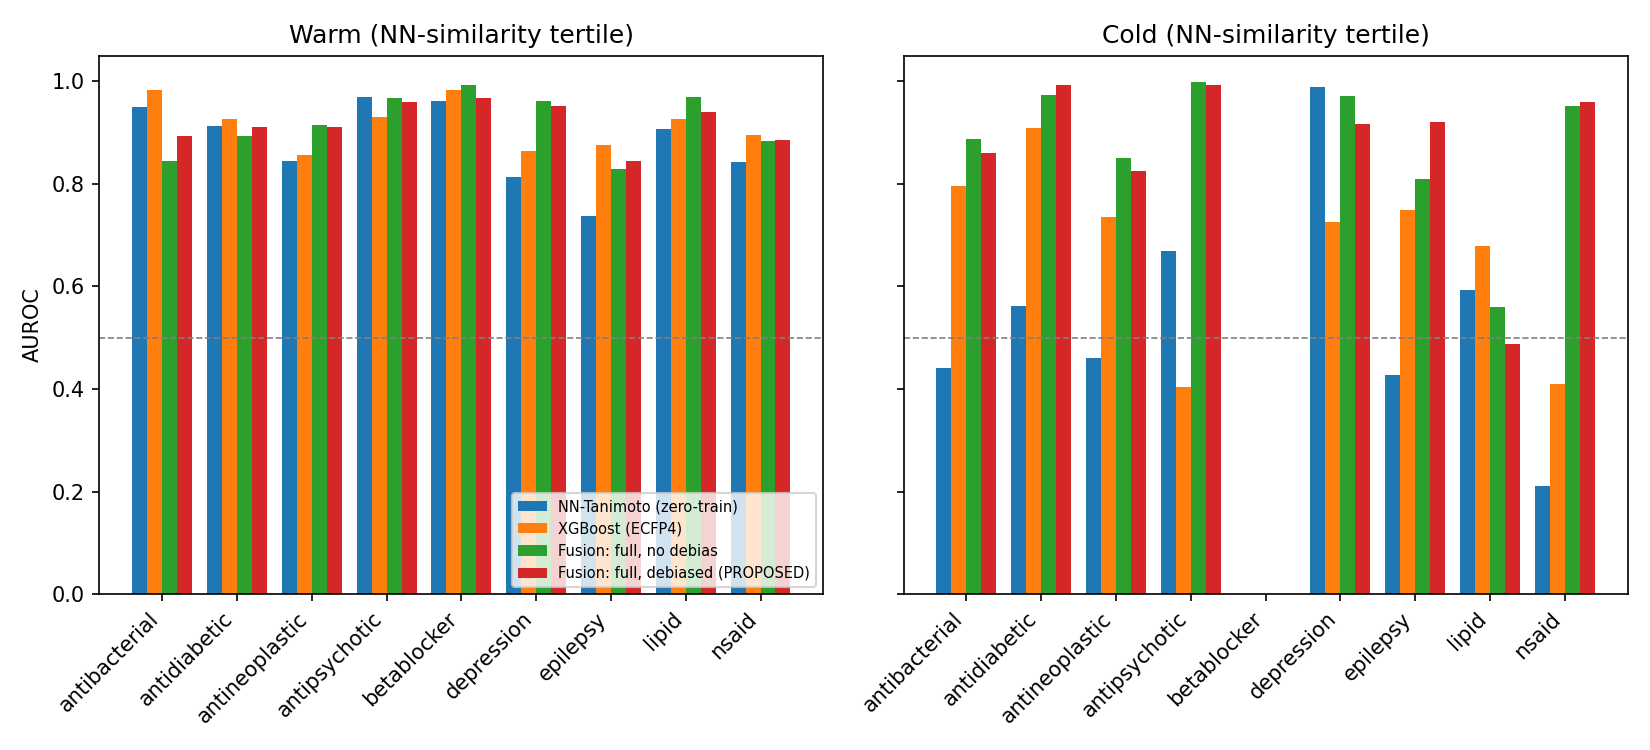
\includegraphics[width=0.95\textwidth]{warm_cold_auroc.png}
\caption{AUROC by class, warm (top similarity tertile) and cold (bottom tertile) test compounds. Betablocker's cold tertile is omitted: its chemistry is dominated by one tight scaffold family, leaving too few genuinely low-similarity compounds to score.}
\label{fig:warmcold}
\end{figure}

Whether fusion\_full improves on fusion\_nodebias in the cold bucket is the real test. Pooling all five seeds before checking misleads, since it hides how many cold-bucket positives back each number. Recomputing the delta per seed rather than pooled surfaces this directly (Table~\ref{tab:cold-reliability}). Three classes, antipsychotics, depression, betablockers, average under one cold-bucket positive per seed, making any AUROC on them uninterpretable regardless of value. Two more, NSAIDs and lipid, remain too data-starved for the sign of their delta to be distinguished from noise.

\begin{table}[t]
\centering
\small
\caption{Cold-bucket debiasing delta (fusion\_full $-$ fusion\_nodebias AUROC), computed per seed rather than pooled, with the mean number of cold-bucket positive examples available per seed. Classes with under $\sim$2 positives per seed on average cannot support a directional claim regardless of the delta shown.}
\label{tab:cold-reliability}
\begin{tabular}{lccc}
\toprule
Class & mean cold $n_{\text{pos}}$/seed & mean delta & std delta \\
\midrule
epilepsy & 6.2 & \textbf{+0.116} & 0.058 \\
antidiabetic & 2.2 & +0.021 & 0.019 \\
antineoplastic & 26.0 & $-$0.024 & 0.048 \\
antibacterial & 6.2 & $-$0.028 & 0.022 \\
nsaid & 1.6 (2/5 seeds usable) & +0.034 & 0.050 \\
lipid & 2.2 & $-$0.083 & 0.176 \\
antipsychotic & 0.4 (0/5 usable) & n/a & n/a \\
depression & 0.2 (0/5 usable) & n/a & n/a \\
betablocker & 0.0 (0/5 usable) & n/a & n/a \\
\bottomrule
\end{tabular}
\end{table}

Four classes have enough cold-bucket positives per seed to say anything. Epilepsy, the class that motivated this study, shows a clear and relatively reliable benefit from debiasing: a mean delta of +0.116 against a standard deviation of 0.058 across five seeds, roughly twice its own noise. Antidiabetic shows a small positive effect of similar reliability. Antibacterial and antineoplastic show modest negative effects. Antineoplastic's delta, despite having the largest cold-bucket sample of any class, 26 positives per seed, is under one standard deviation from zero, so it is not clearly distinguishable from noise either. The defensible claim is narrower than either "debiasing helps across the board" or an unfiltered count of how many classes move in which direction. Debiased reweighting gives a real, meaningful benefit on the motivating class and a smaller one on a second class. It costs a modest and only weakly reliable amount on two more. The remaining five classes simply do not have enough low-similarity examples in this dataset to test the method at all.

As a robustness check, we recomputed the same comparison using the bottom two quintiles instead of the bottom tertile (pooled across seeds, \texttt{results/similarity\_quintile\_auroc.csv}). We ran this specifically to see whether the tertile numbers were a cutoff artifact. They are not: epilepsy's delta is +0.156 on 31 pooled cold-bucket positives, and every other class keeps the sign shown in Table~\ref{tab:cold-reliability}.

\subsection{Leakage audit}
A natural fourth view would be literature about the drug itself, not its target. We show why this is the wrong feature. We start from 33 known antiepileptic drugs and 33 non-antiepileptic drugs approved for antineoplastic or depression indications, and pull PubMed abstracts mentioning each drug's name, restricted to strictly before its own approval year. 7 of 66 candidates, mostly pre-1960s drugs with sparse MEDLINE coverage, had no usable pre-approval text and were dropped, leaving 30 and 29. A TF-IDF logistic regression, five-fold cross-validated, predicts the eventual antiepileptic label from this pre-approval text at 0.959 AUROC (Figure~\ref{fig:leakage}). Masking obvious disease-defining terms (\emph{epilep*}, \emph{seizur*}, \emph{anticonvulsant*}, \emph{antiepileptic*}, \emph{convulsant*}, \emph{convulsion*}, \emph{AEDs?}) barely changes this, 0.953. The masked model's driving coefficients are almost entirely names of other antiepileptic drugs: lorazepam, midazolam, diazepam, carbamazepine, gabapentin, valproate, clonazepam, vigabatrin. The text predicts the label not through pharmacology but because papers about a future antiepileptic already co-mention other, already-approved antiepileptics as comparators. That is the same leakage mechanism documented for diagnosis codes in clinical prediction~\cite{labelleakage2023jamia,labelleakage2025jama}, transposed to drug-name co-occurrence, and it is why we exclude drug-literature text rather than rely on a held-out split to catch it.

\begin{figure}[t]
\centering
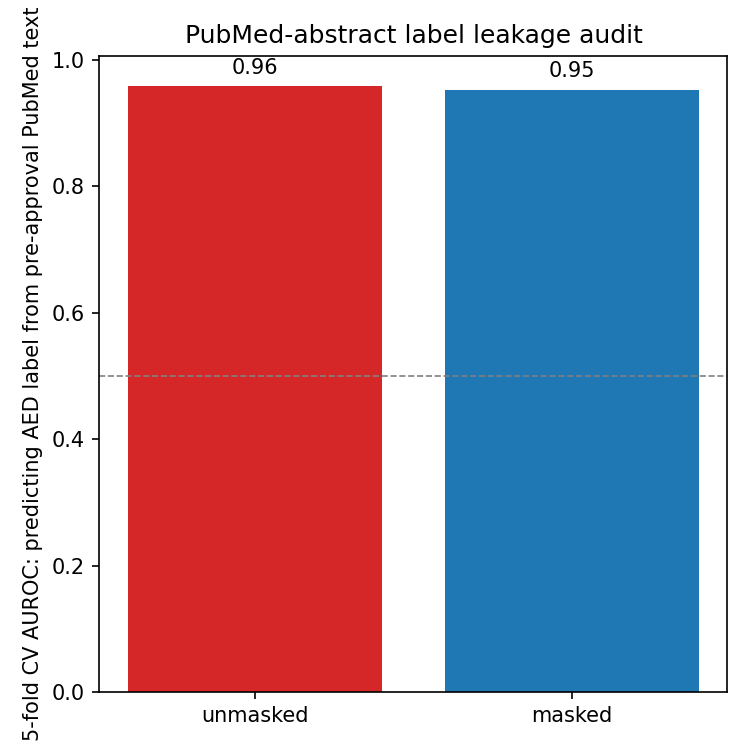
\includegraphics[width=0.6\textwidth]{leakage_audit.png}
\caption{Five-fold cross-validated AUROC for predicting a drug's eventual antiepileptic label from PubMed abstracts published strictly before its own approval date, with and without disease-defining terms masked ($n=59$).}
\label{fig:leakage}
\end{figure}

\subsection{Biological-interpretation positive control}
\label{sec:moa}
A real AUROC gain could come from a feature artifact, not anything pharmacologically sensible. So we check whether the debiased model's top cold-bucket picks make mechanistic sense, using a field never seen during training: the Broad Repurposing Hub's mechanism-of-action (MoA) string. No input references this field directly, though the text view's UniProt description and the MoA string both trace to the same target, so only chemistry and expression are fully independent of it. We first validate the check. Of the 34 known antiepileptic drugs in our data, 18 resolve to a Hub MoA entry, and 14 of those (78\%) contain one of \emph{GABA}, \emph{sodium channel}, \emph{calcium channel}, \emph{glutamate}, \emph{potassium channel}, or \emph{SV2A}. That is against a 7.8\% base rate across the full MoA table, a roughly tenfold enrichment on drugs with a known mechanism.

We restrict to the cold bucket and to true negatives, excluding already-known antiepileptics so the check cannot rediscover training labels. Within that set, we take each seed's top 50 candidates and compute this same keyword-hit rate.

\begin{table}[t]
\centering
\small
\caption{Top-50 cold-bucket MoA-keyword hit rate (mean $\pm$ std, 5 seeds), against the cold-bucket candidate base rate.}
\label{tab:moa}
\begin{tabular}{lcc}
\toprule
Model & Top-50 rate & \\
\midrule
nn\_tanimoto & 0.004 & $\pm$0.009 \\
fusion\_nodebias & 0.228 & $\pm$0.039 \\
fusion\_full (proposed) & \textbf{0.300} & $\pm$0.028 \\
cold-bucket base rate & 0.013 & $\pm$0.001 \\
\bottomrule
\end{tabular}
\end{table}

The nearest-neighbor guide does worse than chance here, consistent with its cold-bucket collapse in Section~\ref{sec:experiments}. With no close structural neighbor, its top 50 carries no mechanistic signal. Both fusion variants recover a large, non-circular enrichment, 17 to 23 times the base rate, from structure, expression, and target-function text alone. Debiasing adds a further, consistent lift over the already-large undebiased enrichment, 0.300 against 0.228, same direction across all five seeds. That corroborates the AUROC-based debiasing delta in Section~\ref{sec:experiments}, from a label never used as a training target.

A separate concern: epilepsy positives carry a Hub annotation far more often than negatives, 22/31 vs. 2{,}264/9{,}847, so the gain could reflect mere annotation presence, not content. We test this by shuffling real embeddings among annotated compounds while holding true availability fixed. That collapses the fusion model to the no-text level, 0.648 vs. 0.647, and single-view text drops below chance. The gain tracks content, not availability (\texttt{code/text\_availability\_shortcut\_check.py}).

\subsection{External validation of the epilepsy delta on an independent label source}
\label{sec:repodb}
The epilepsy delta rests entirely on ChEMBL-derived labels, the only indication source used anywhere in this paper. We checked it against repoDB~\cite{brown2017repodb}, an approved-indication resource built from DrugCentral, independent of ChEMBL. 32 drugs carry an Approved epilepsy indication there, 23 of which resolve to a LINCS compound. Of those, 20 (87\%) already carry our ChEMBL-derived positive label, a reassuring cross-source agreement. 3 are new positives ChEMBL missed, and 11 ChEMBL positives are unconfirmed by repoDB's older, differently-vocabularied snapshot.

We swap the evaluation label on the already-frozen out-of-fold scores, with no retraining. repoDB yields only 5 unique cold-bucket positives, the same 5 across all seeds, 4 already ChEMBL-positive: mostly the same drugs under a second label, not a fresh sample. The ChEMBL-label delta on this row set reproduces the headline +0.115; the repoDB-label delta is $-0.002 \pm 0.072$. With only 5 positives, swapping one compound, repoDB adds pyridoxine and drops newer AEDs it predates, moves the AUROC by the full effect size either way. That is a power limit, not a design choice. The broader premise survives: nn\_tanimoto still collapses below chance (0.359), and both fusion variants still reach $\approx$0.86 absolute AUROC. The +0.116 increment does not survive this check. We treat this as a limit on how much weight that number carries, not a refutation, since 5 positives cannot refute anything.

\subsection{External validation on an expanded, LINCS-decoupled candidate pool}
\label{sec:expanded}
The repoDB check in Section~\ref{sec:repodb} is underpowered by only 5 compounds. We built a second, better-powered check instead: extending the epilepsy candidate pool beyond the 9{,}878-compound LINCS library to the full ChEMBL-derived label set adds 25 new positives with no L1000 profile, for 56 total against the original 31, and 8.8 cold-bucket positives per seed against 6.2.

On this expanded pool, the same training configuration, confirmed near-optimal by held-out validation AUROC independent of the cold-bucket metric, gives a mean cold-bucket delta of $-0.001$ across five seeds, not +0.116, stable across three reruns at different initializations ($-0.015$ to $-0.037$). Restricting the expanded pool back to exactly the original 31 LINCS-covered positives reproduces +0.090 (std 0.036), close to the committed +0.116: the benefit holds for the compounds it was built on and fails specifically on the 25 new ones that lack a real expression profile and are routed around that view by the model's gate. This does not generalize as a rule; antibacterial's delta moves the opposite direction under the same expansion ($-0.031$ to $+0.074$). The scope boundary we can state with confidence is specific to epilepsy: the benefit requires a complete three-view profile and has not been shown to extend to candidates missing one.

\subsection{Empirical comparison against adapted DRDM and TAPB baselines}
\label{sec:baselines}
Neither debiasing method named in Related Work transfers to this task as its own architecture. DRDM's GNN was built for curated drug-disease benchmarks with thousands of diseases, and TAPB's correction is built around protein-target embeddings this task does not have. We instead implement the bias-correction \emph{mechanism} of each, adapted to our nine-indication label set (full detail in \texttt{code/drdm\_baseline.py} and \texttt{code/tapb\_baseline.py}), and evaluate both on the identical epilepsy cold-bucket split used throughout. DRDM's annealed inverse-degree edge reweighting becomes a two-hop bipartite graph model over the nine label sets. TAPB's confounder-cluster backdoor adjustment becomes a clustering of the nine indications' positive-rate scores, with per-cluster predictions combined by a shared classifier. Both share a feature-based drug encoder with the rest of the pipeline, trained jointly across all nine indications: TAPB's correction requires that joint structure, and DRDM gets the same setup rather than less data.

\begin{table}[t]
\centering
\small
\caption{Epilepsy cold-bucket AUROC (mean $\pm$ std, 5 seeds): adapted DRDM and TAPB baselines against this paper's own models.}
\label{tab:baselines}
\begin{tabular}{lc}
\toprule
Model & Cold-bucket AUROC \\
\midrule
nn\_tanimoto & 0.425 $\pm$ 0.016 \\
drdm\_adapted & 0.433 $\pm$ 0.190 \\
tapb\_adapted & 0.852 $\pm$ 0.018 \\
multitask\_control (joint training, no debiasing) & 0.863 $\pm$ 0.009 \\
fusion\_nodebias & 0.799 $\pm$ 0.053 \\
fusion\_nodebias, joint-trained control & 0.797 $\pm$ 0.015 \\
fusion\_full (proposed) & \textbf{0.915} $\pm$ 0.052 \\
\bottomrule
\end{tabular}
\end{table}

The DRDM-style baseline recovers no usable signal, 0.433 mean AUROC, indistinguishable from the nearest-neighbor guide. It is also an order of magnitude noisier across seeds, std 0.190 against 0.016--0.058 elsewhere in this paper, consistent with a mechanism that needs a far denser association graph than nine indications and roughly 470 total edges can support. The TAPB-style baseline recovers strong, stable signal, 0.852. But a control isolating why, the same joint drug encoder with a plain linear head and no confounder-cluster correction, matches it almost exactly, 0.863. TAPB's correction adds nothing measurable beyond what joint multi-indication training already supplies. Its apparent strength is a multi-task-learning effect, not evidence for its own mechanism. Our proposed model, with no joint multi-indication training, still reaches the highest point estimate, 0.915. That margin over the multitask control, though, sits within roughly one standard deviation of fusion\_full's own seed-to-seed noise, and should be read as suggestive, not decisive. A matched control, same architecture and hyperparameters, varying only training regime, scores 0.797 $\pm$ 0.015 jointly trained against 0.799 $\pm$ 0.053 per-task: indistinguishable.

\section{Discussion and Limitations}
The central premise holds. A zero-training chemical-similarity search accounts for most of a repurposing model's apparent accuracy, and that accuracy is close to or below chance on the novel-scaffold compounds a repurposing method is meant to find. Debiased reweighting against this shortcut is not a uniform fix across therapeutic areas in our implementation. It gives a real, meaningfully-sized benefit on the class that motivated the study, a smaller one on a second class, and a modest, weakly-reliable cost or too few low-similarity examples to test on the rest. This honest, uneven result is more useful than either extreme, so we report the per-class breakdown rather than one pooled number. The epilepsy delta holds under the ChEMBL label but is not confirmed by a repoDB check limited to 5 compounds (Section~\ref{sec:repodb}). The premise and enrichment both survive that check, while the +0.116 number remains real under its original construction and unresolved beyond it. A second, better-powered check (Section~\ref{sec:expanded}) sharpens this: the delta reproduces on the original LINCS-covered pool but collapses on candidates missing an expression profile, so the benefit is real but scoped to a complete three-view profile. Section~\ref{sec:baselines}'s adapted-baseline comparison confirms the proposed model still holds the best point estimate. It also surfaces a transferable pitfall: TAPB looks strong mainly because of joint multi-indication training, not its own correction, as a plain-head multitask control reveals. Any benchmark adapting a correction method that also changes the training regime needs this control before crediting the correction to its stated mechanism. A matched check on our own gated-fusion encoder shows no such boost, 0.797 against 0.799 per-task, so the confound may be specific to TAPB's simpler encoder rather than universal. The need for this control, not the confound itself, is what generalizes.

Several limitations should guide how much weight the current numbers carry. The fusion model encodes every view, including the 2{,}048-dim ECFP4 view, through an MLP, while the strongest plain-chemistry baseline (xgb\_ecfp) uses a tree ensemble. Table~\ref{tab:headline} shows it beating fusion\_struct, the MLP-only ablation, on most classes. The fusion variants are not controlled against xgb\_ecfp, so part of the full model's margin over it may reflect the extra views, not architecture. All results come from one library (LINCS) and one indication source (ChEMBL). Section~\ref{sec:baselines}'s DRDM/TAPB comparisons adapt each mechanism to our label structure, not its original architecture, since neither transfers as-is to a task with no protein-target axis (TAPB) or a graph this sparse (DRDM). Table~\ref{tab:baselines} bounds what we could test, not either method's own-benchmark performance. Chemprop now matches the paper's five-seed, five-fold protocol, reaching 0.852, near lr\_ecfp and below xgb\_ecfp/fusion\_full. TxGNN was not run, an unsatisfiable pinned dependency rather than a missing checkpoint, and the guide used 5 CV repeats, not DebiasedDTA's 10. Pooled bootstrap intervals treat non-independent resamples as independent, understating uncertainty; claims rest on per-seed mean and std instead. The 59-drug leakage audit is also small: the conclusion is clear, but the estimate is imprecise. Code: \url{https://github.com/edanmn/debiased-drug-repurposing}.

\bibliographystyle{splncs04}
\bibliography{refs}

\end{document}
